\documentclass[11pt,english]{article}

\setlength{\oddsidemargin}{0cm}
\setlength{\topmargin}{-2cm}
\setlength{\textwidth}{160mm}
\setlength{\textheight}{230mm}

\usepackage[english]{babel}                      
\usepackage[utf8]{inputenc}                    
\usepackage{amsmath}                             
\usepackage{amssymb}                               
\usepackage[pdftex]{graphicx}                    
\usepackage{float} 
\usepackage{subfigure} 
\usepackage[ruled,linesnumbered]{algorithm2e}
\usepackage[colorlinks, linkcolor=blue]{hyperref}
\usepackage{appendix}

\DeclareGraphicsExtensions{.jpg,.mps,.pdf,.png}    

\begin{document}

\title
{
    \textbf{Project DAAR \\ Mark-Compact GC for MINIZAM in C\\}
}

\author
{
    \\
    \\
    \\
    \\
    \\
    Submitted by
    \\
    \\
    \textbf{Hejun Cao}
    \\
    \textbf{Ruolin Zhou}
    \\
    \textbf{Weida Liu}
    \\
    \\
    M1 Science et Technologie du Logiciel 2023-2024
    \\
    Sorbonne Universite (SU UMPC)
    \\
    \\
    \\
    Under the guidance of 
    \\
    \\
    \textbf{\href{https://www-npa.lip6.fr/~buixuan/}{\textcolor{black}{Bùi Xuân Bình Minh}}}
    \\
    Sorbonne Universite (SU UPMC)
}

\date{20/01/2025}

\maketitle

\begin{figure}[h]
    \begin{center}
        
\includegraphics[height=3cm]{./src/logo_lip6.png}
    \end{center}
\end{figure}

\begin{figure}[h]
    \begin{center}
        
\includegraphics[height=3cm]{./src/Science_Sorbonne_logo.png}
    \end{center}
\end{figure}

\pagebreak

\tableofcontents

\pagebreak
\large{
    \section{Introduction}
    
    \indent

    Dans le cadre de notre projet DAAR, nous avons choisi de développer une application web/mobile de moteur de recherche 
    pour une bibliothèque numérique, conformément aux exigences du "CHOIX A". 
    Ce projet s'inscrit dans un contexte où les bases de données textuelles de grande envergure, comme la bibliothèque de Gutenberg, 
    rendent la recherche manuelle inefficace. L'objectif principal est donc de concevoir une solution performante 
    et intuitive permettant aux utilisateurs de localiser efficacement des documents textuels au sein d'une bibliothèque comprenant au minimum 1664 livres, 
    chaque livre contenant au moins 10 000 mots.

    \indent
    Le projet s'articule autour de plusieurs objectifs clés :

    \begin{itemize}
        \item Un système de gestion des utilisateurs.
        \\
        Pour gérer les recommandations personnalisées uniques de chaque utilisateur et le tri des résultats de recherche, ainsi que la fonction de favoris correspondante.
        
        \item KMP Search.
        \\
        La recherche de contenu par expressions régulières à l'aide de KMP Search appris dans les cours de DAAR permet de trouver tous les contenus textuels de tous les livres et les résultats sont triés en fonction du nombre d'occurrences.
    
        \item Recommandation de contenu.
        \\
        Nous utilisons l'algorithme PageRank pour calculer le score PageRank de chaque nœud (livre) dans le graphe de similarité des livres, les livres ayant un score élevé étant considérés comme les plus appréciés par l'utilisateur, tout en filtrant les résultats en fonction de l'auteur et de la catégorie afin de nous assurer que les livres recommandés correspondent aux intérêts de l'utilisateur.
    
    \end{itemize}

    \indent En plus des défis techniques liés à l'implémentation des algorithmes de recherche et de classement, une attention particulière sera portée à la performance de l'application, mesurée à travers des tests sur des volumes de données conséquents. 


    \section{Implémentation détaillée}

    \subsection{Gestion des utilisateurs}


    \indent

    Notre module utilisateur met en œuvre les fonctions d'enregistrement, de connexion, de modification et de déconnexion des utilisateurs, ainsi que les fonctions de collecte de livres.

    \indent Nous avons mis en œuvre des modules utilisateurs pour la protection des bases de données à l'aide de filtres de Bloom, de verrous distribués, de buckets limitant les flux et de la mise en cache Redis.

    \begin{figure}[H]
        \begin{center}
            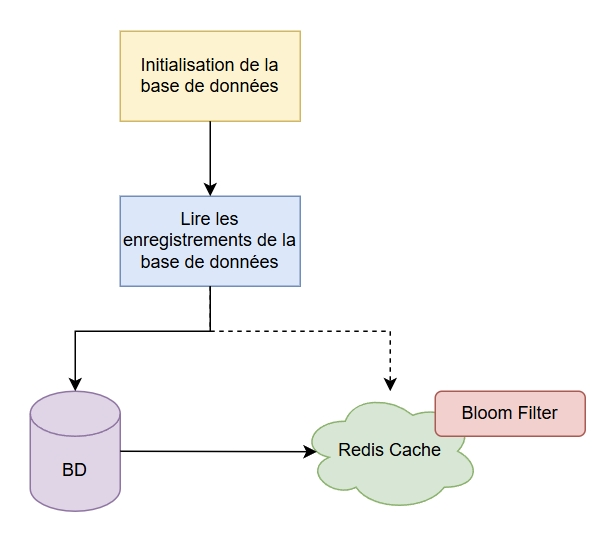
\includegraphics[height=9cm]{./src/DB_Init.png}
        \end{center}
    \end{figure}

    \indent À chaque fois que le projet s'exécute, nous lisons d'abord les données de la base de données, puis nous les synchronisons avec le cache Redis pour nous assurer qu'il n'y a pas de doublons.

    \indent Entre-temps, nous avons conçu les solutions suivantes pour faire face à d'éventuelles attaques de bases de données :
    S'il y a un grand nombre d'appels à l'interface d'enregistrement/de connexion avec le même nom d'utilisateur, nous utiliserons d'abord des filtres Bloom pour le filtrage, puis des verrous distribués pour verrouiller les noms d'utilisateur afin de garantir qu'une seule demande peut interroger la base de données en même temps.

    \begin{figure}[H]
        \begin{center}
            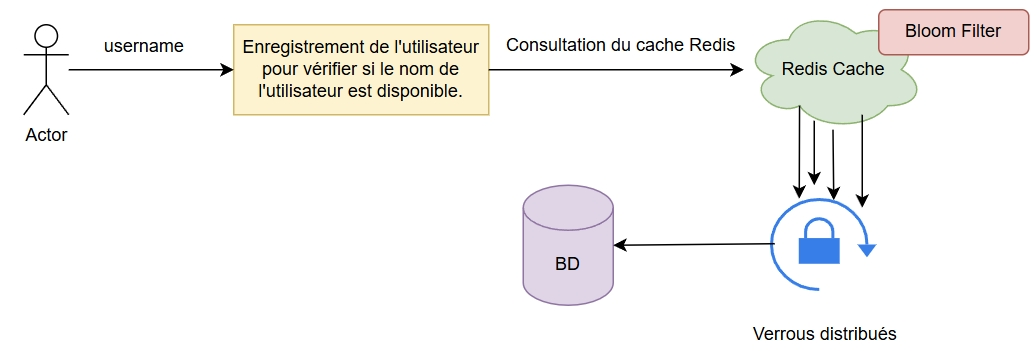
\includegraphics[height=5.4cm]{./src/user_regis.png}
        \end{center}
    \end{figure}

    \indent En outre, nous avons mis en place une fonction de collecte facile. L'utilisateur crée un groupe et y place le livre correspondant. Les données du livre dans la collection affectent le poids de l'algorithme PageRank.

    \subsection{KMP Search}

    \subsubsection{Analyse}

    \indent

    L'algorithme de Knuth-Morris-Pratt, également connu sous le nom d'algorithme KMP, est un algorithme de correspondance de chaînes de caractères. Son idée de base est que lorsqu'il y a une non-concordance de chaîne, vous pouvez savoir quelle partie du texte doit correspondre.

    \indent L'idée centrale de l'algorithme KMP est d'utiliser des informations connues pour réduire autant que possible le nombre de correspondances. Plus précisément, il peut être divisé en deux étapes :

    \indent Compute le tableau Carryover et puis utilise KMP Search.

    \subsubsection{Structure de donnees}

    \indent 

    Comme pour le Projet précédent, nous lisons toujours le texte entier, ligne par ligne, et nous le recherchons. Par conséquent, sa structure de données est une simple chaîne de caractères.

    \subsubsection{Implémentation}

    \indent 
    
    L'algorithme KMP peut générer un tableau LST à partir d'une chaîne de motifs prétraitée, puis convertir le tableau LST en un tableau de report, où report[i] indique la position à laquelle la chaîne de motifs doit sauter pour poursuivre la comparaison si le i-ème caractère de la chaîne de motifs ne correspond pas à un caractère de la chaîne de texte.

    \indent 

    \begin{algorithm}[H]
        \caption{ComputeCarryover}\label{alg:computeCarryover}
        
        \textbf{Inputs}
            character array \\
        \textbf{Outputs}
            The final $LST$ array\\
        \textit{Calculations}\\
            \For{$i \gets 0$ to $len - 1$ by $1$}{
                \If{$j == -1$ OR $pattern[i] == pattern[j]$}{
                    $i \gets i + 1$ \\
                    $j \gets j + 1$ \\
                    $LST[i] \gets j$
                }
                \Else{
                    $j \gets next[j]$
                }
            }
            \For{$i \gets 1$ to $len$ by $1$}{
                \If{$LST[i] \geq 0$ and $i < len$ and $pattern[i] == pattern[LST[i]]$}{
                    $LST[i] \gets LST[LST[i]]$
                }
            }
    \end{algorithm}

    \indent L'algorithme utilise une table de sauts précalculée (carryover) pour gérer efficacement le processus de correspondance. Chaque fois qu'une correspondance échoue, l'algorithme ajuste rapidement le pointeur de motif à travers la table de saut pour continuer à rechercher une correspondance. Si une correspondance est réussie, elle est enregistrée et le pointeur est réinitialisé pour poursuivre la recherche de l'occurrence suivante. Enfin, le contenu correspondant est renvoyé.

    \indent 

    \begin{algorithm}[H]
        \caption{KPM (Knuth-Morris-Pratt)}\label{alg:kpm}
        \textit{Inputs}
        \begin{itemize}
            \item[$\bullet$] $factor = $ a string (the pattern to search for)
            \item[$\bullet$] $file = $ a string (the file path)
        \end{itemize}
        \textit{Initializations}
        \begin{itemize}
            \item[$\bullet$] $factorChar = $ Convert $factor$ to a character array
            \item[$\bullet$] $carryover = $ Result of calling $computeCarryover(factorChar)$
            \item[$\bullet$] $lineNumber = 0$
        \end{itemize}
        \textit{Calculations}\\
        \While{there is a new line in the file}{
            $lineNumber \gets lineNumber + 1$ \\
            $line = $ read the next line from the file \\
            $i \gets 0$, $j \gets 0$ \\
            $textLen = $ length of $line$ \\
            $factorLen = $ length of $factorChar$
            
            \While{$i < textLen$}{
                \If{$j == -1$ OR $line[i] == factorChar[j]$}{
                    $i \gets i + 1$ \\
                    $j \gets j + 1$
                    \If{$j == factorLen$}{
                        $j \gets carryover[j]$ 
                    }
                }
                \Else{
                    $j \gets carryover[j]$
                }
            }
        }
        \textit{Outputs}
        \begin{itemize}
            \item[$\bullet$] The matches found in the file (if any) with the corresponding line number
        \end{itemize}
    \end{algorithm}

    \subsection{PageRank}

    \subsubsection{Analyse}
    
    \indent 

    L'algorithme PageRank a été proposé à l'origine par Larry Page et Sergey Brin pour mesurer l'importance des pages web. L'idée de base est que s'il y a beaucoup de pages de haute qualité (PageRank élevé) qui pointent vers une page, alors cette page a plus de chances d'être de haute qualité. Mathématiquement, le PageRank peut être considéré comme une sorte de « distribution à l'état stable » sur un graphique, modélisant la distribution de probabilité d'un spectateur aléatoire qui continue à cliquer sur des hyperliens ou à passer aléatoirement d'un nœud à l'autre pour atteindre d'autres nœuds.

    \indent Pour un graphe orienté contenant N nœuds, la valeur de PageRank de chaque nœud i est désignée par PR$(i)$ et la formule itérative de base pour PageRank peut être écrite :

    \begin{center}
        $PR(i) = \frac{1 - d}{N} + d \sum_{j \in \mathrm{In}(i)} \frac{PR(j)}{\mathrm{OutDegree}(j)}$
    \end{center}

    \indent Parmi eux:

    \begin{itemize}
        \item d est le facteur d'amortissement, généralement 0,85, ce qui signifie que dans le modèle de marche aléatoire, la probabilité d'utiliser un lien hypertexte pour continuer à sauter est d, tandis que la probabilité de sauter vers n'importe quel nœud directement et aléatoirement sans utiliser de lien hypertexte est de 1 - d.
        \item N est le nombre total de nœuds.
        \item In(i) désigne l'ensemble des nœuds dont l'arête pointe vers i (c'est-à-dire les voisins entrants de i).
        \item OutDegree(j) indique le degré de sortie du nœud j (c'est-à-dire le nombre d'arêtes partant du nœud j).
    \end{itemize}

    \indent Dans l'algorithme PageRank, si un nœud n'a pas d'arêtes sortantes (outdegree 0), toute sa valeur PageRank ne peut pas être transmise à d'autres nœuds par le biais de « liens ».

    \indent PageRank est un algorithme itératif :

    \begin{itemize}
        \item Commencez par donner à tous les nœuds une valeur initiale.(Par example 1/N)
        \item Il est ensuite mis à jour de manière itérative selon la formule. Jusqu'à ce que la différence entre les deux itérations précédentes et suivantes soit inférieure à un certain seuil ou que le nombre maximal d'itérations soit atteint, la convergence est considérée comme atteinte et l'itération est arrêtée.
    \end{itemize}

    \subsubsection{Structure de donnees}

    \indent 
    
    Dans la mise en œuvre du PageRank de ce projet, les quatre types suivants de structures de données centrales sont utilisés pour construire et traiter efficacement des structures de graphe à grande échelle :

    \begin{itemize}
        \item Liste d'adjacence positive
        \\Définition de la structure : Map$<$Long, List$<$Long$>$$>$ graph
        \\Signification : Key représente l'identifiant du noeud (dans ce projet, il correspond à l'identifiant du livre), Value est une liste contenant les identifiants de tous les noeuds vers lesquels ce noeud pointe (ou auxquels il est similaire).

        \item Liste d'adjacence inversée
        \\\textbf{Définition de la structure :} Map$<$Long, List$<$Long$>>$ reverseGraph
        \\\textbf{Signification :} la clé représente l'identifiant du noeud, la valeur est l'ensemble des « autres identifiants de noeuds pointant vers ce noeud ».

        \item Carte des degrés de sortie (Out-degree Map)
        \\\textbf{Définition de la structure :}  Map$<$Long, Integer$>$ outDegreeMap
        \\\textbf{Signification :} Enregistrer la relation de correspondance entre l'identifiant du nœud et son degré de sortie (nombre d'arêtes sortantes).

        \item Stockage du PageRank (PageRank Map)
        \\\textbf{Définition de la structure :}Map$<$Long, Double$>$ pageRank
        \\\textbf{Signification :}Enregistre le score PageRank actuel de chaque noeud.
    \end{itemize}

    \subsubsection{Implémentation}

    \indent

    Nous devons d'abord construire la table de voisinage inverse et la table des degrés sortants.
    
    \begin{algorithm}[H]
        \SetAlgoLined
        \caption{Build Reverse Graph}
        \KwIn{$graph$: A map where each key is a node, and the value is a list of its outgoing neighbors.}
        \KwOut{$reverseGraph$: A map where each key is a node, and the value is a list of its incoming neighbors.}
        
        \SetKwData{ReverseGraph}{reverseGraph}
        \SetKwData{Graph}{graph}
        \SetKwData{Node}{node}
        \SetKwData{OutNodes}{outNodes}
        
        \ReverseGraph $\gets$ empty map with lists as values\;
        \ForEach{\Node $\in$ \Graph.keys()}{
            \ReverseGraph.put(\Node, empty list)\;
        }
        \ForEach{\Node $\in$ \Graph.keys()}{
            \OutNodes $\gets$ \Graph.get(\Node)\;
            \If{\OutNodes is not null}{
                \ForEach{outNode $\in$ \OutNodes}{
                    \ReverseGraph.get(outNode).add(\Node)\;
                }
            }
        }
        \Return{\ReverseGraph}\;
    \end{algorithm}

    \begin{algorithm}[H]
        \SetAlgoLined
        \caption{Build Out-Degree Map}
        \KwIn{$graph$: A map where each key is a node, and the value is a list of its outgoing neighbors.}
        \KwOut{$outDegreeMap$: A map where each key is a node, and the value is the count of its outgoing neighbors.}
        
        \SetKwData{OutDegreeMap}{outDegreeMap}
        \SetKwData{Graph}{graph}
        \SetKwData{Node}{node}
        \SetKwData{OutList}{outList}
        \SetKwData{OutDegree}{outDegree}
        
        \OutDegreeMap $\gets$ empty map\;
        \ForEach{\Node $\in$ \Graph.keys()}{
            \OutList $\gets$ \Graph.get(\Node)\;
            \OutDegree $\gets$ (\OutList is null) ? 0 : \OutList.size()\;
            \OutDegreeMap.put(\Node, \OutDegree)\;
        }
        \Return{\OutDegreeMap}\;
    \end{algorithm}

    \indent

    L'idée spécifique de la mise en œuvre de notre algorithme est la suivante :

    \indent Nous commençons par déterminer si le graphe d'entrée est vide. Si le graphe est vide ou n'a pas de nœuds, il renvoie directement le résultat null. Cela permet d'éviter les exceptions de pointeur nul dans les calculs ultérieurs.

    \indent Les structures de données auxiliaires (graphe inversé et carte des degrés de sortie) sont ensuite construites.

    \indent Ensuite, nous attribuons une valeur initiale de PageRank à chaque nœud PR(\text{node}) = $\frac{1}{N}$ dont N est le nombre total de nœuds, ce qui indique que tous les nœuds ont la même importance initiale.

    \indent Nous calculons ensuite la contribution des nœuds en suspens et répartissons la valeur du PageRank de tous les nœuds en suspens de manière égale entre tous les nœuds du graphe selon la formule suivante.

    \begin{center}
        $\text{danglingSum} = \sum_{\text{node} \in \text{graph.keys()}, \text{outDegree[node]} = 0} PR(\text{node})$
    \end{center}

    \indent La contribution de chaque nœud au nœud suspendu est alors $\frac{\text{danglingSum}}{N}$.

    \indent Immédiatement après, nous mettons à jour le PageRank nœud par nœud et, pour chaque nœud, nous calculons la nouvelle valeur du PageRank à l'aide de la formule :

    \begin{center}
        $PR(\text{node}) = \frac{1 - d}{N} + d \cdot \frac{\text{danglingSum}}{N} 
        + d \cdot \sum_{\text{inNode} \in \text{reverseGraph[node]}} 
        \frac{PR(\text{inNode})}{\text{outDegree[inNode]}}
        $
    \end{center}

    \indent Enfin, nous calculons le changement total entre cette itération et l'itération précédente :
    
    \begin{center}
        $\text{diff} = \sum_{\text{node} \in \text{graph.keys()}} 
        \left| PR_{\text{new}}(\text{node}) - PR_{\text{old}}(\text{node}) \right|
        $
    \end{center}

    \indent Si diff<$\epsilon $, les valeurs de PageRank sont considérées comme convergentes et l'itération peut être arrêtée prématurément pour renvoyer les valeurs de PageRank de tous les nœuds.

    \begin{algorithm}[H]
        \SetAlgoLined
        \caption{Compute PageRank}
        \KwIn{$graph$: A map where keys are book IDs, values are lists of directly connected book IDs. \\
        $dampingFactor$: Damping coefficient, typically set to 0.85. \\
        $maxIterations$: Maximum number of iterations. \\
        $epsilon$: Convergence threshold, used to terminate early if the difference between two iterations is small.}
        \KwOut{$pageRank$: A map where keys are book IDs and values are their corresponding PageRank scores.}
        
        \If{$graph$ is null or empty}{
            \Return{empty map}\;
        }
        
        % Step 1: Build reverse graph and out-degree map
        $reverseGraph \gets$ \textbf{BuildReverseGraph}($graph$)\;
        $outDegreeMap \gets$ \textbf{BuildOutDegreeMap}($graph$)\;
        
        $nodeCount \gets$ size of $graph$\;
        $pageRank \gets$ map initialized to $1.0 / nodeCount$ for each node\;
        
        % Step 2: Iterative computation of PageRank
        \For{$iter \gets 0$ \textbf{to} $maxIterations - 1$}{
            % Step 2.1: Calculate the total rank from dangling nodes
            $danglingSum \gets 0.0$\;
            \ForEach{$node \in graph.keys()$}{
                \If{$outDegreeMap[node] = 0$}{
                    $danglingSum \gets danglingSum + pageRank[node]$\;
                }
            }
        
            % Step 2.2: Compute new PageRank for each node
            $newPageRank \gets$ empty map\;
            \ForEach{$node \in graph.keys()$}{
                $rank \gets \frac{1.0 - dampingFactor}{nodeCount} + dampingFactor \cdot \frac{danglingSum}{nodeCount}$\;
                $inNeighbors \gets reverseGraph[node]$\;
                \If{$inNeighbors$ is not empty}{
                    \ForEach{$inNode \in inNeighbors$}{
                        $outDeg \gets outDegreeMap[inNode]$\;
                        \If{$outDeg > 0$}{
                            $rank \gets rank + dampingFactor \cdot \frac{pageRank[inNode]}{outDeg}$\;
                        }
                    }
                }
                $newPageRank[node] \gets rank$\;
            }
        
            % Step 2.3: Check for convergence
            $diff \gets$ \textbf{CalculateDifference}($pageRank, newPageRank$)\;
            $pageRank \gets newPageRank$\;
            \If{$diff < epsilon$}{
                \textbf{break}\;
            }
        }
        \Return{$pageRank$}\;
    \end{algorithm}
        
        

    \section{Tests et Résultats}


    \subsection{KMP Search}

    \indent 
    
    Nous avons testé les performances de l'algorithme KMP ainsi que l'optimisation multithreading et les résultats sont présentés dans la Fig.

    \begin{figure}[H]
        \begin{center}
            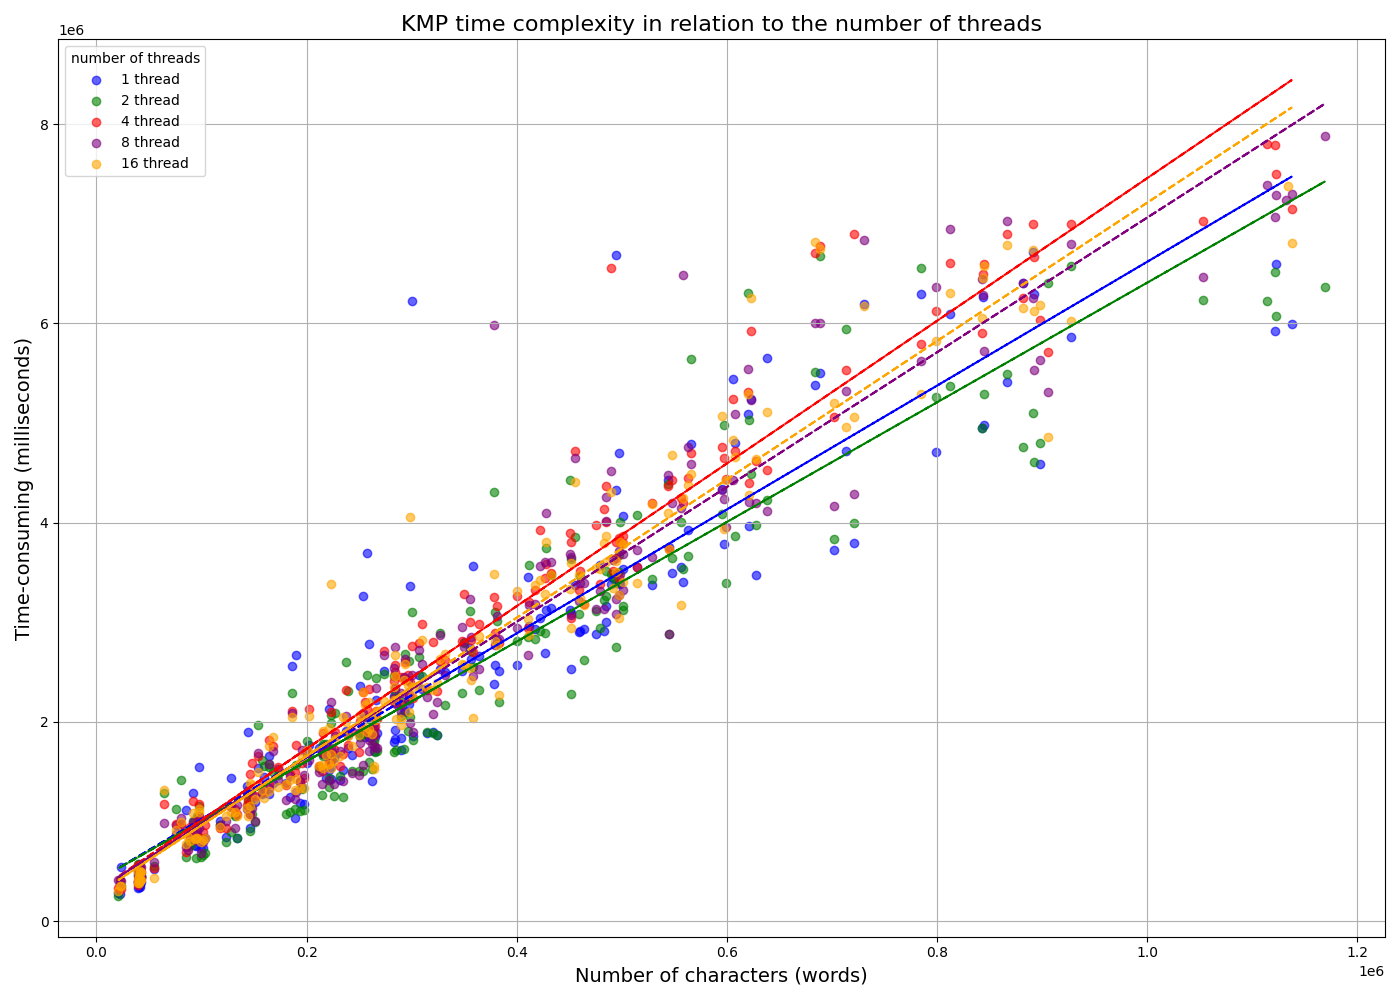
\includegraphics[height=9cm]{./src/KMP_Multi.png}
        \end{center}
    \end{figure}

    \indent On peut constater intuitivement qu'une simple lecture multithread ligne par ligne n'a pas beaucoup d'impact sur la recherche KMP, parce que chaque ligne de texte n'a pas beaucoup de contenu et qu'il est difficile pour le multithreading d'obtenir un avantage significatif dans une tâche aussi petite.

    \indent Ensuite, nous avons essayé de diviser le texte entier en X parties, X étant le nombre total de fils, et les résultats du test sont présentés dans la figure.

    \begin{figure}[H]
        \begin{center}
            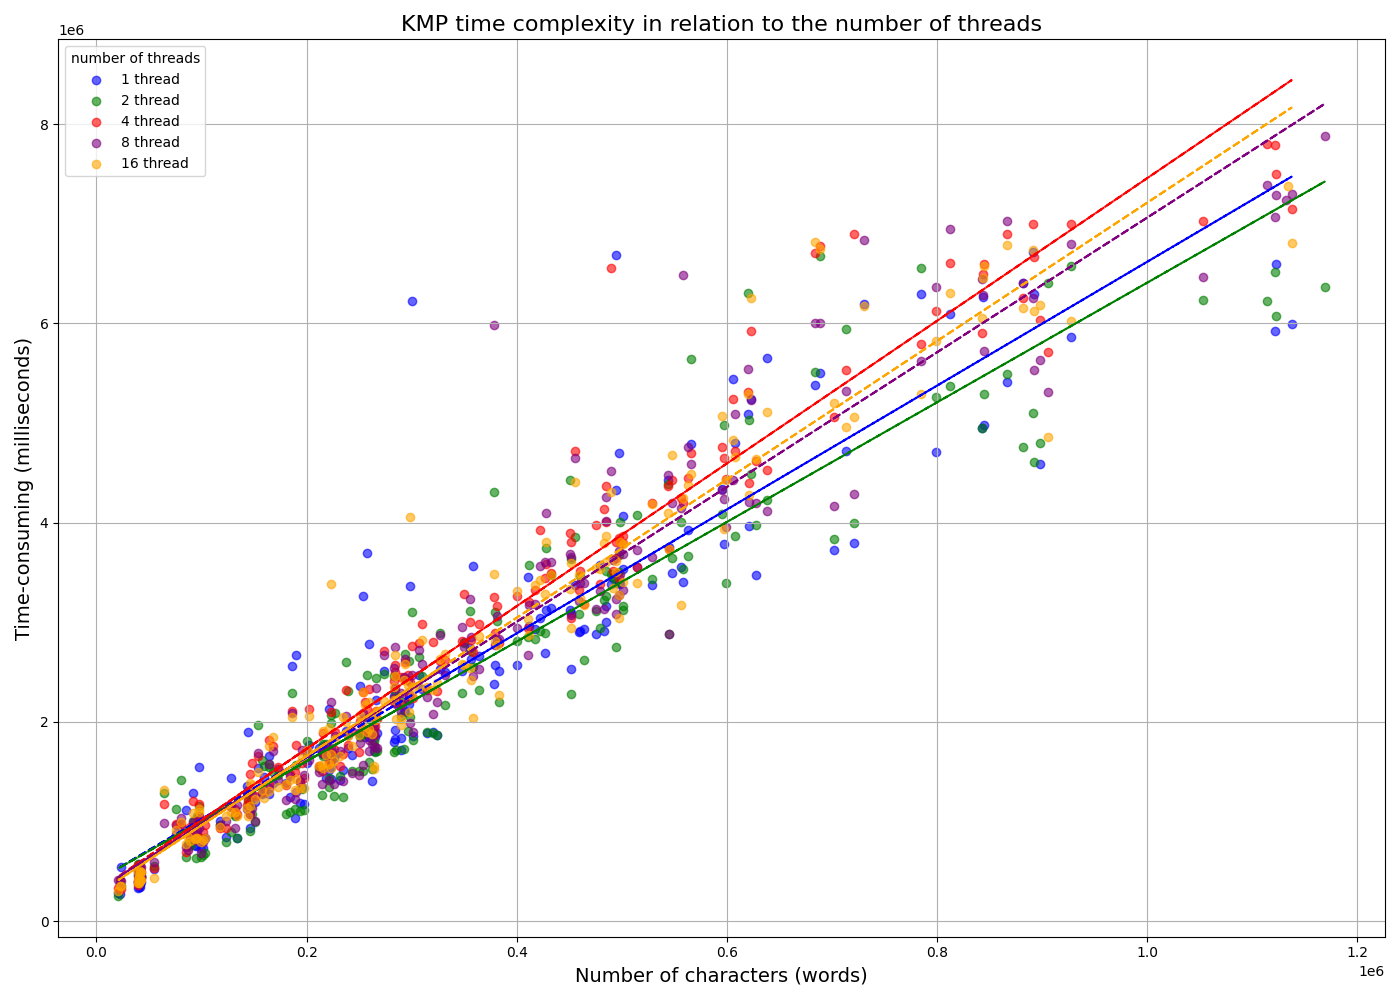
\includegraphics[height=9cm]{./src/KMP_Multi_Part.png}
        \end{center}
    \end{figure}

    \indent Là encore, l'impact du multithreading n'est pas évident.

    \indent Enfin, nous avons également essayé d'optimiser le processus de recherche avec ES Search. Voici les résultats de la comparaison des performances entre ES Search et KMP Search.

    \begin{figure}[H]
        \begin{center}
            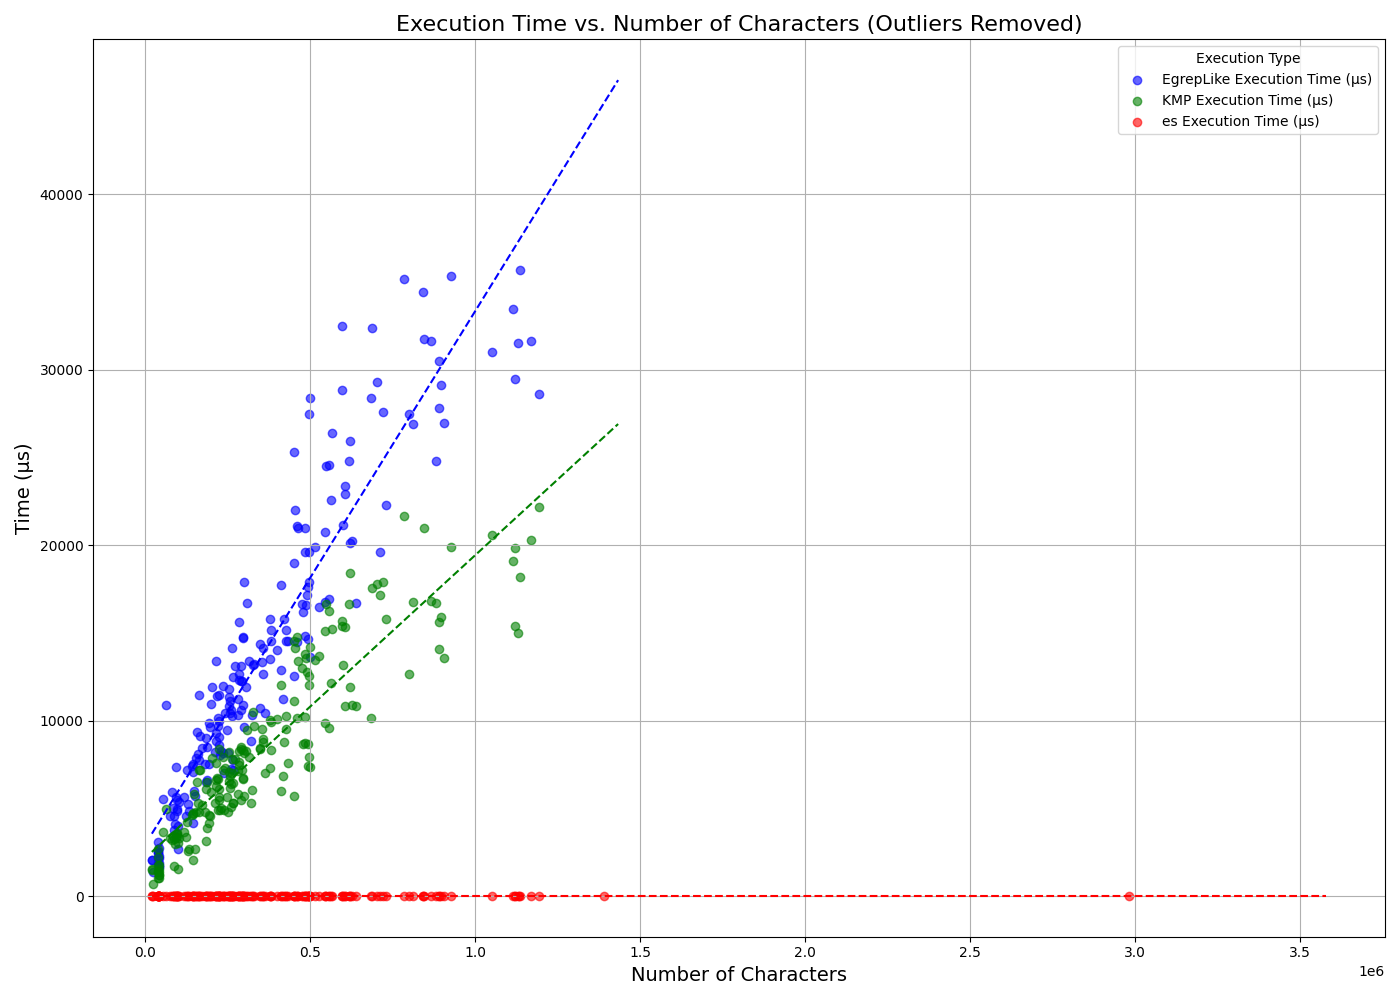
\includegraphics[height=9cm]{./src/ES_VS_KMP.png}
        \end{center}
    \end{figure}

    \indent 

    \subsection{PageRank}

    \indent

    Les recommandations de livres varient en fonction des collections de l'utilisateur. Par exemple, lorsque l'utilisateur n'a pas de collection, la recommandation de livre ressemble à ceci :
    
    \begin{figure}[H]
        \begin{center}
            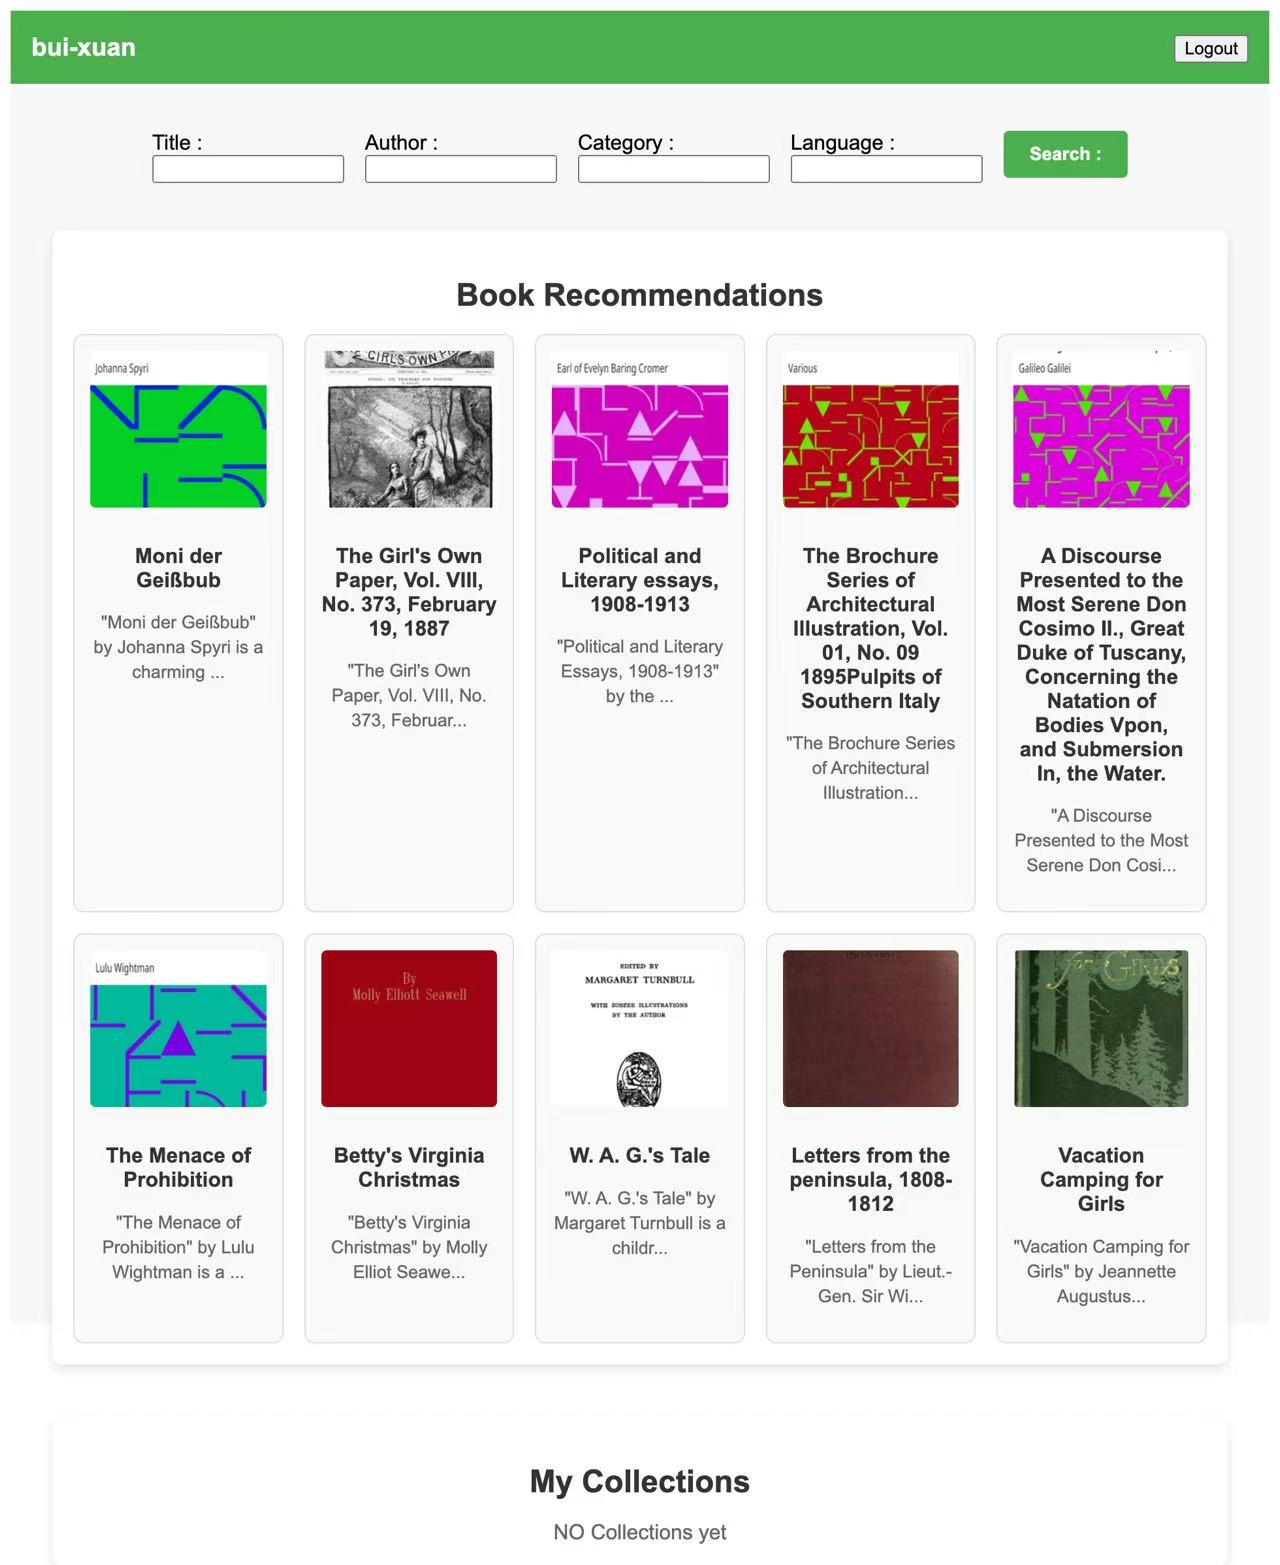
\includegraphics[height=9cm]{./src/Rank1.jpg}
        \end{center}
    \end{figure}

    \indent Lorsque l'utilisateur a d'autres livres dans sa collection, nous faisons des recommandations personnalisées différentes basées sur la catégorie/l'auteur/la langue du livre collecté :

    \begin{figure}[H]
        \begin{center}
            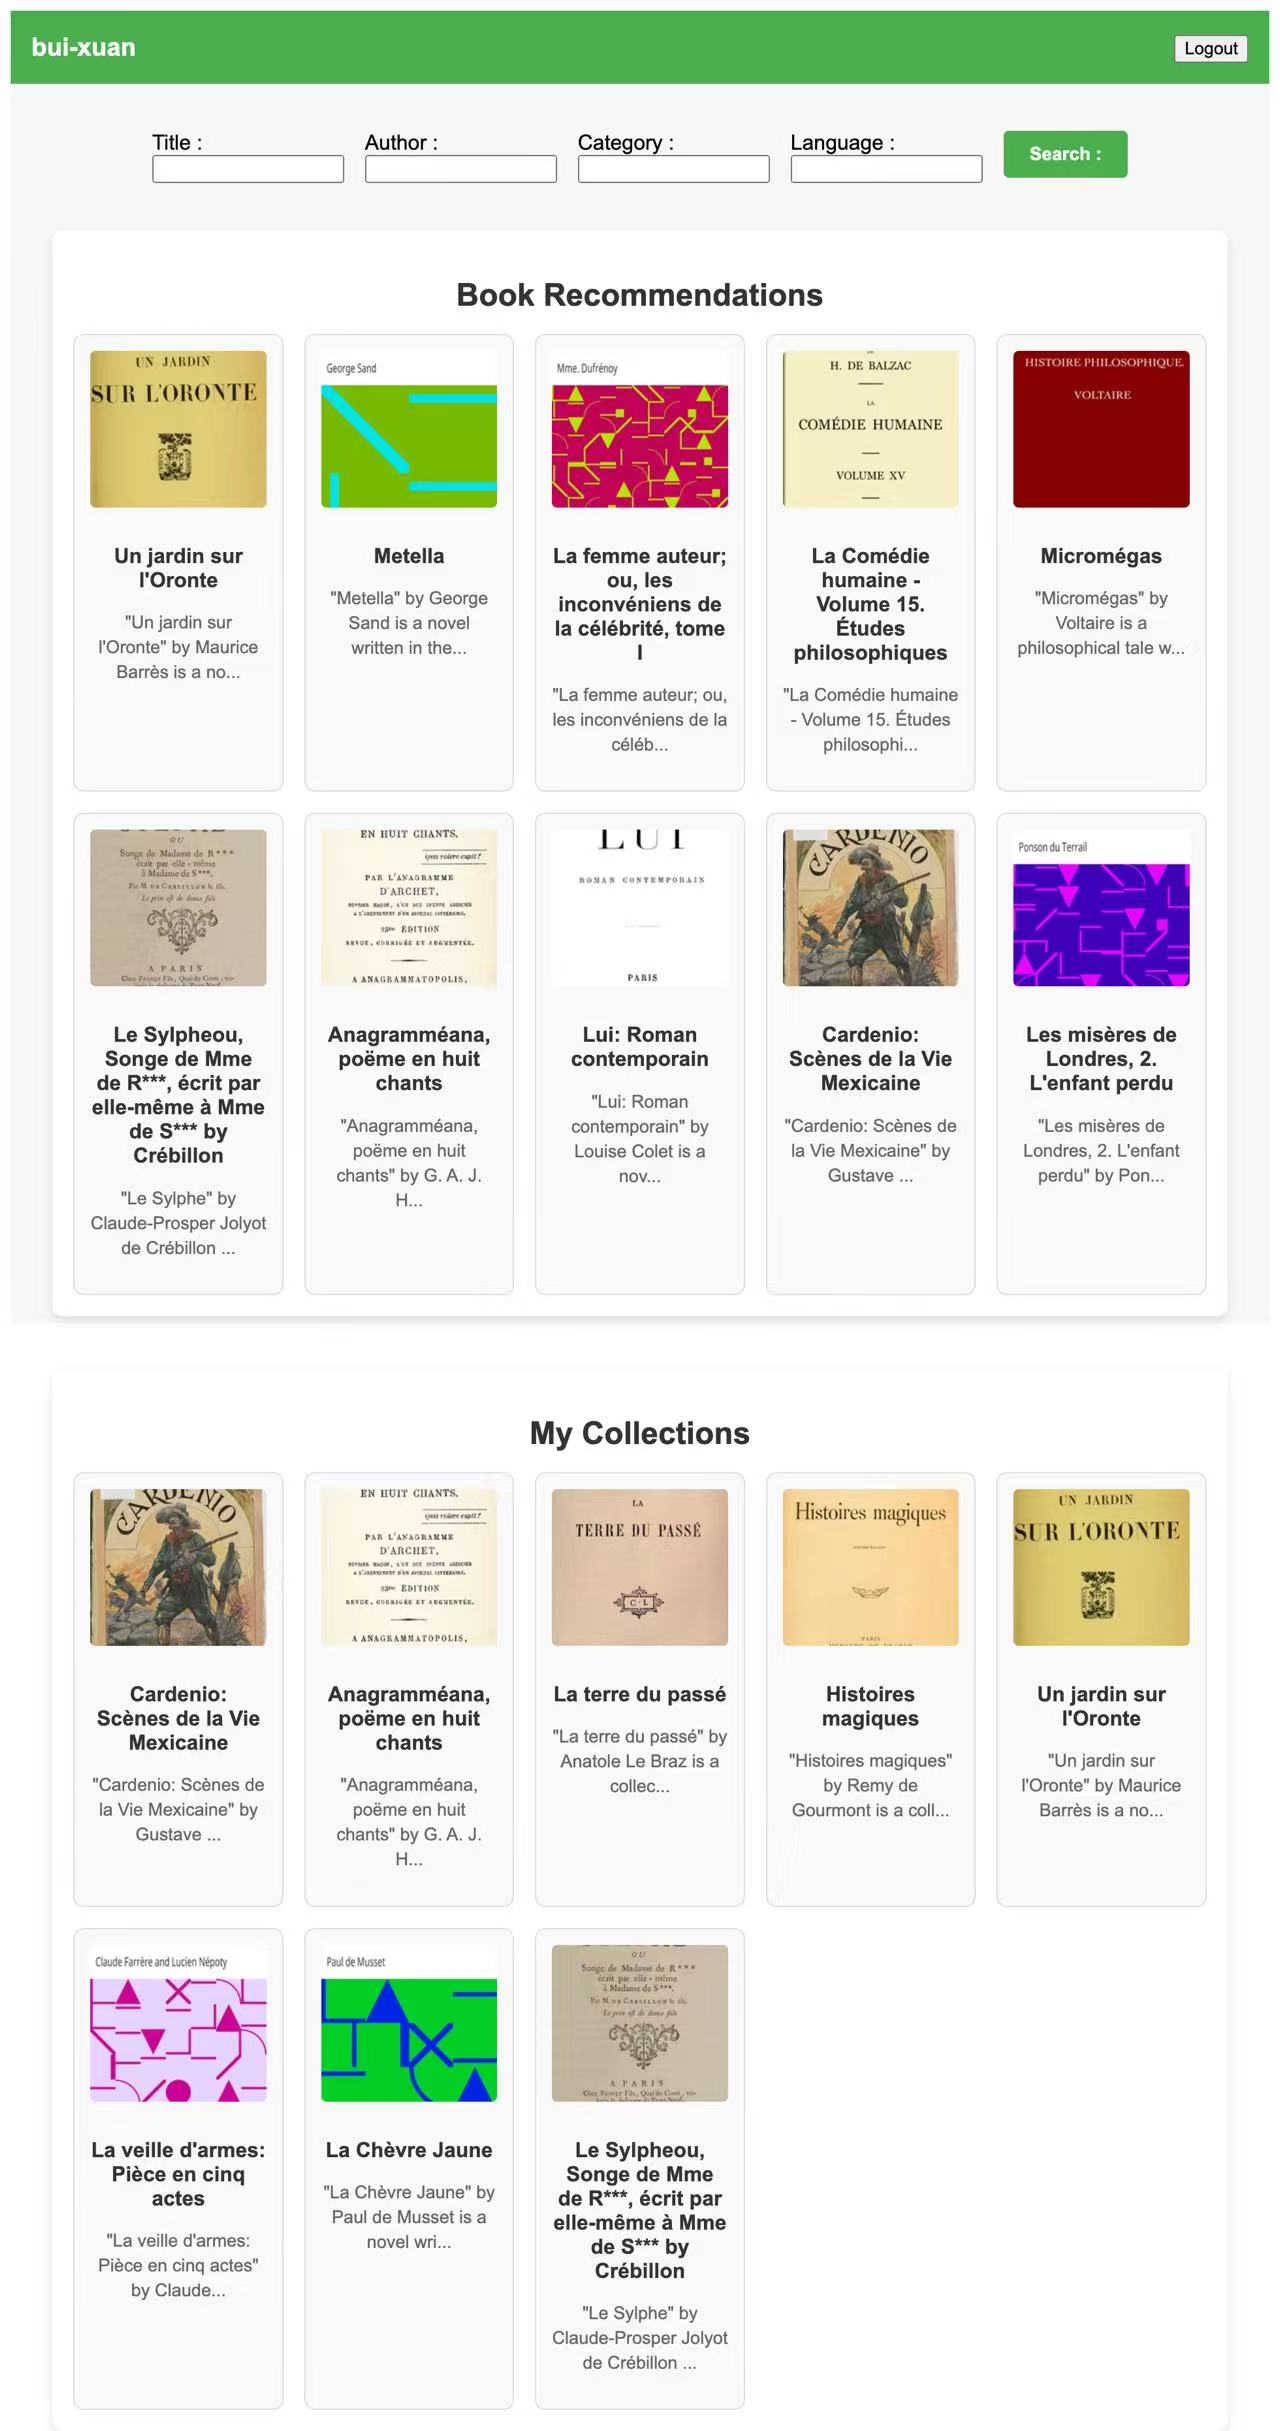
\includegraphics[height=9cm]{./src/Rank3.jpg}
        \end{center}
    \end{figure}


    \section{Conclusion}

    \indent

    Dans le cadre de ce projet DAAR, nous avons conçu et développé un moteur de recherche performant pour une bibliothèque numérique, intégrant des techniques avancées de gestion de données et d'optimisation des performances. En mettant en œuvre des algorithmes tels que KMP pour la recherche de texte et PageRank pour la recommandation de contenu, nous avons assuré une navigation efficace et pertinente au sein d'une vaste collection de documents.

    \indent L'intégration d'un système de gestion des utilisateurs a permis de personnaliser l'expérience en fonction des préférences et des interactions des utilisateurs, garantissant ainsi une meilleure pertinence des résultats de recherche et des recommandations. Les tests réalisés ont mis en évidence les performances et les limites de nos choix d'implémentation, notamment en ce qui concerne l'efficacité du multithreading pour la recherche KMP et l'impact des collections d’utilisateurs sur les recommandations.

    \indent En conclusion, notre projet a démontré la faisabilité et l'efficacité d'une approche algorithmique rigoureuse pour la gestion de bibliothèques numériques de grande échelle. Des perspectives d'amélioration existent, notamment en explorant d'autres stratégies d'optimisation et en intégrant des modèles d'apprentissage automatique pour affiner encore davantage les recommandations et la recherche textuelle.
}
\end{document}